\subsection{M.PC.1 - Percentuale di metriche soddisfatte}
\begin{figure}[H]
    \centering
    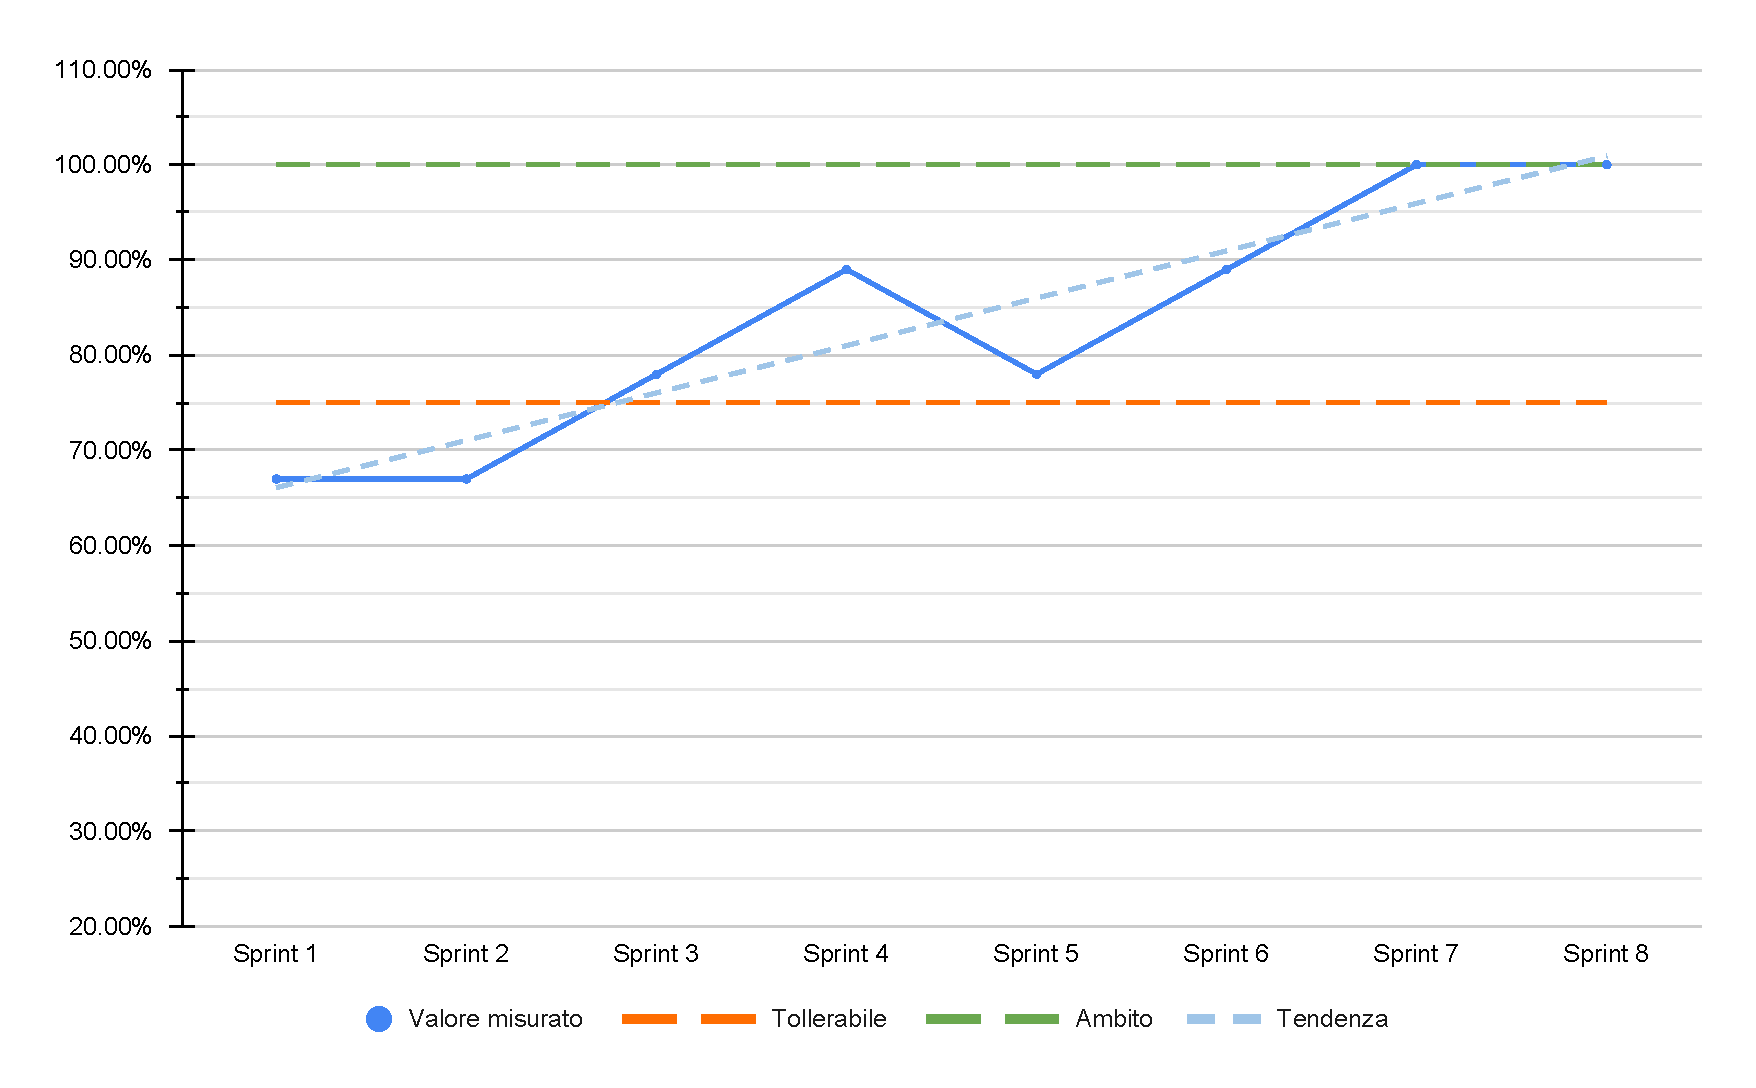
\includegraphics[width=\textwidth]{assets/metriche_soddisfatte.pdf}
    \caption{M.PC.1 - Percentuale di metriche soddisfatte}
\end{figure}

\par Il grafico sottolinea come negli \glossario{sprint} iniziali il team non abbia raggiunto la soglia di tollerabilità stabilita. Il mancato raggiungimento degli obiettivi era dovuto all’inesperienza del team e alla difficoltà di adattamento ai processi di lavoro e alle pratiche dell’ingegneria del software. Tuttavia, nel corso degli \glossario{sprint} successivi, il gruppo ha notato dei progressi, specie nell’ottemperanza alle metriche di variazione del piano e del budget. Questo è dovuto all'introduzione di feedback migliorativi, alla maggiore competenza e collaborazione all'interno del team, e all’applicazione più puntuale del ciclo di PDCA. Inoltre, il gruppo ha aggiornato e approfondito il \WoW\ nelle \NdP, incrementando la qualità dei processi. Il grafico illustra un miglioramento costante nel tempo, fino a raggiungere il valore ambito alla fine del sesto sprint. Già dal quarto sprint, però, il valore misurato era superiore alla soglia considerata tollerabile. L’obiettivo del team è di riuscire a mantenere un livello di qualità costante anche quando verrà introdotta la misurazione delle metriche di prodotto.
